\chapter{Análisis de datos ingestados en el lago de datos}

En este apartado, se busca realizar una serie de consultas analíticas para demostrar al cliente cómo poder extraer información relevante para su caso de uso. Además, también se busca demostrar cómo persistir datos agregados en una nueva tabla para poder ser consultados de manera más rápida por herramientas de BI o de Dashboarding.

\section{Consultas}

\subsection{Preparación de las consultas}

Para poder ejecutar las consultas vamos a cargar los dataframes que hemos guardado en el lago de datos:

\begin{lstlisting}[language=scala]
import java.util.Properties
val properties = new Properties()

properties.setProperty("user", "postgres")
properties.setProperty("driver", "org.postgresql.Driver")
properties.setProperty("password", "postgres")
properties.setProperty("partitionColumn", "altitude")
properties.setProperty("lowerBound", "0")
properties.setProperty("upperBound", "2000")
properties.setProperty("numPartitions", "10")
properties.setProperty("password", "postgres")

val df_airports = spark.read.option("partitionColumn", "altitude").option("lowerBound", 0).option("upperBound", 2000).option("numPartitions", 10).jdbc("jdbc:postgresql://localhost:5432/postgres", "airports", properties)

val df_airlines = spark.read.format("parquet").load("hdfs://localhost:9000/practica/airlines/")
val df_countries = spark.read.format("csv").option("header", "true").option("inferSchema", "true").load("hdfs://localhost:9000/practica/countries/")

val df_routes=spark.read.format("org.apache.spark.sql.cassandra").option("spark.cassandra.connection.host","127.0.0.1").option("spark.cassandra.connection.port","9042").option("keyspace", "practica").option("table", "routes").load()
\end{lstlisting}

Ahora pasaremos los dataframes a \texttt{TempViews} para poder realizar consultas SQL sobre ellos:

\begin{lstlisting}[language=scala]
df_airports.createOrReplaceTempView("airports")
df_airlines.createOrReplaceTempView("airlines")
df_countries.createOrReplaceTempView("countries")
df_routes.createOrReplaceTempView("routes")
\end{lstlisting}

\begin{figure}[H]
    \centering
    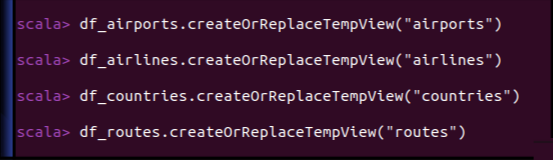
\includegraphics[width=0.8\textwidth]{figures/59.png}
    \caption{Creación de las vistas temporales de los dataframes}
    \label{fig:tempviews}
\end{figure}

\subsection{Consulta 1}

La primera consulta que se nos pide es obtener los aeropuertos con mayor altitud. Para ello, se ha realizado la siguiente consulta:

\begin{lstlisting}[language=scala]
spark.sql("SELECT * FROM airports ORDER BY altitude DESC LIMIT 1").show()
\end{lstlisting}

\begin{figure}[H]
    \centering
    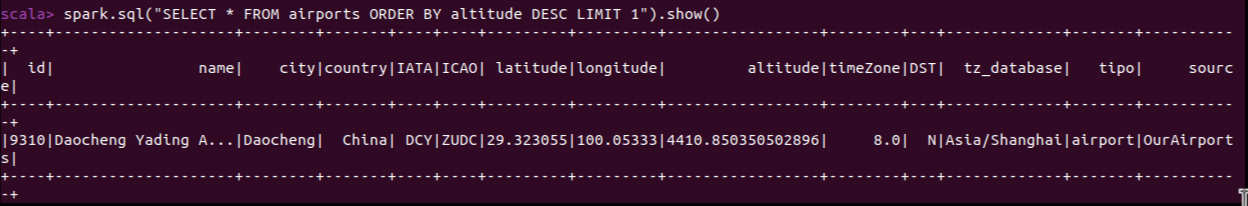
\includegraphics[width=0.8\textwidth]{figures/60.png}
    \caption{Resultado de la consulta de aeropuertos con mayor altitud}
    \label{fig:consulta1}
\end{figure}

\subsection{Consulta 2}

La segunda consulta que se nos pide es obtener el número de aeropuertos que hay en España. Para ello, se ha realizado la siguiente consulta:

\begin{lstlisting}[language=scala]
spark.sql("SELECT COUNT(country) AS airport_count FROM airports WHERE country == 'Spain'").show()
\end{lstlisting}

\begin{figure}[H]
    \centering
    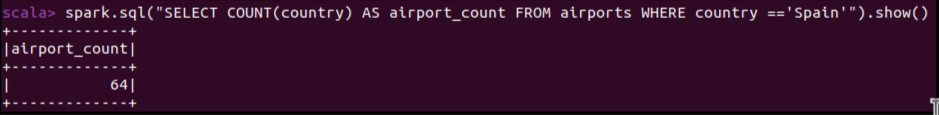
\includegraphics[width=0.8\textwidth]{figures/61.png}
    \caption{Resultado de la consulta de aeropuertos en España}
    \label{fig:consulta2}
\end{figure}

\subsection{Consulta 3}

La tercera consulta que se nos pide es obtener los países que tienen aeropuertos cuyo horario de verano sea el de Europa. Para ello, se ha realizado la siguiente consulta:

\begin{lstlisting}[language=scala]
spark.sql("SELECT DISTINCT country FROM airports WHERE dst == 'E'").show()
\end{lstlisting}

\begin{figure}[H]
    \centering
    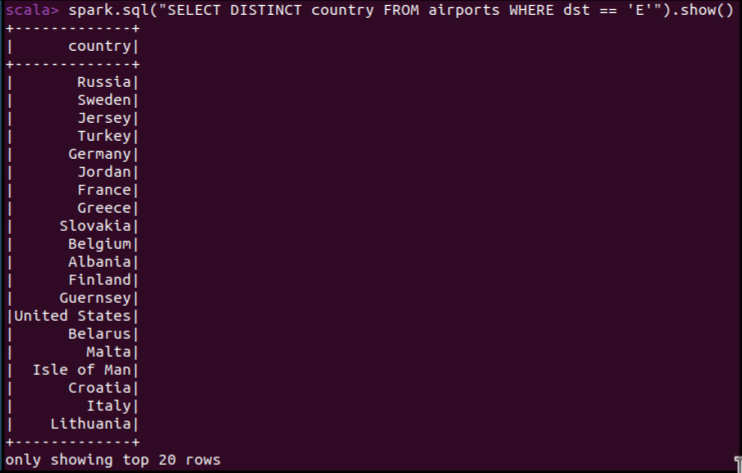
\includegraphics[width=0.8\textwidth]{figures/62.png}
    \caption{Resultado de la consulta de países con aeropuertos en horario de verano de Europa}
    \label{fig:consulta3}
\end{figure}

\subsection{Consulta 4}

La cuarta consulta que se nos pide es obtener el número de aerolíneas que tiene EEUU. Como habíamos particionado los datos por país, cargaremos los datos de las aerolíneas de EEUU y contaremos el número de filas:

\begin{lstlisting}[language=scala]
val df_airlines_usa = spark.read.format("parquet").option("header","true").option("inferSchema", "true").load("hdfs://localhost:9000/practica/airlines/country=United States")
df_airlines_usa.count()
\end{lstlisting}

\begin{figure}[H]
    \centering
    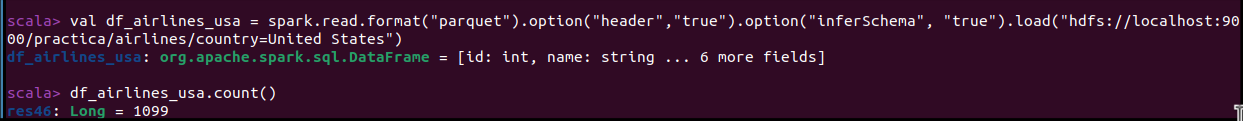
\includegraphics[width=0.8\textwidth]{figures/69.png}
    \caption{Resultado de la consulta de aerolíneas en EEUU con particionado por país}
    \label{fig:consulta4-1}
\end{figure}

También se puede realizar la consulta directamente con SQL:

\begin{lstlisting}[language=scala]
spark.sql("SELECT COUNT(*) AS airline_count FROM airlines WHERE country == 'United States'").show()
\end{lstlisting}

\begin{figure}[H]
    \centering
    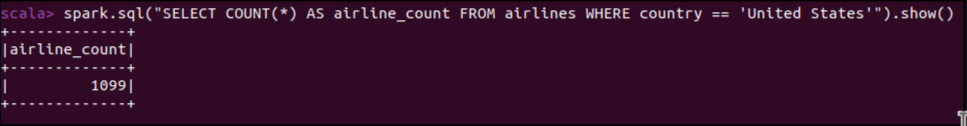
\includegraphics[width=0.8\textwidth]{figures/63.png}
    \caption{Resultado de la consulta de aerolíneas en EEUU}
    \label{fig:consulta4-2}
\end{figure}

\subsection{Consulta 5}

La quinta consulta que se nos pide es obtener los 10 países con más aerolíneas inactivas. Para ello, se ha realizado la siguiente consulta:

\begin{lstlisting}[language=scala]
spark.sql("SELECT country, COUNT(*) AS inactive_airlines FROM airlines WHERE active == 'f' GROUP BY country ORDER BY inactive_airlines DESC LIMIT 10").show()
\end{lstlisting}

\begin{figure}[H]
    \centering
    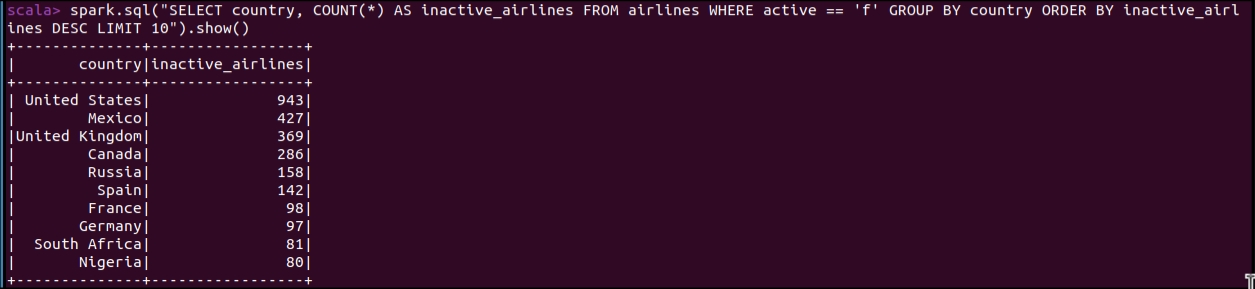
\includegraphics[width=0.8\textwidth]{figures/64.png}
    \caption{Resultado de la consulta de países con más aerolíneas inactivas}
    \label{fig:consulta5}
\end{figure}

\subsection{Consulta 6}

La sexta y última consulta que se nos pide es obtener los países que tienen aerolíneas en activo y aeropuertos con una latitud mayor a 80. Para ello, se ha realizado la siguiente consulta:

\begin{lstlisting}[language=scala]
spark.sql("SELECT DISTINCT a.country FROM airports a JOIN airlines b ON a.country = b.country WHERE a.latitude > 80 AND b.active == 't'").show()
\end{lstlisting}

\begin{figure}[H]
    \centering
    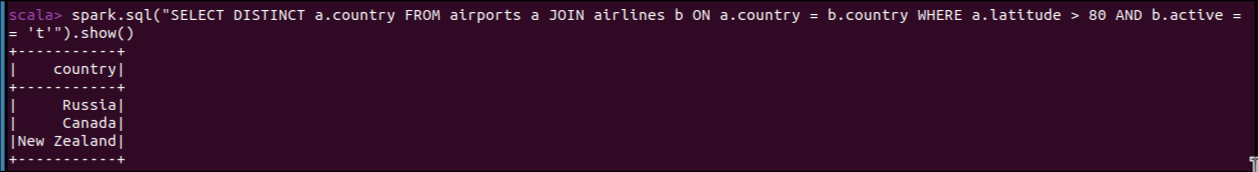
\includegraphics[width=0.8\textwidth]{figures/65.png}
    \caption{Resultado de la consulta de países con aerolíneas activas y aeropuertos con latitud mayor a 80}
    \label{fig:consulta6}
\end{figure}

\section{Persistencia de datos agregados}

Por último, también queremos mostrar al cliente la capacidad que tiene nuestra plataforma para guardar datos agregados en tablas nuevas para poder realizar informes o consultar datos específicos con menor procesamiento y menor latencia. 

Para ello, se necesita crear una tabla llamada aggregations que guarde sus datos en formato
parquet en la ruta /practica/aggregations/ de HDFS y que responda a la siguiente pregunta:

- ¿Cuántas rutas sin paradas (stops) a destinos con una altitud (altitude) mayor a 200 metros
se hicieron por país (country) con aerolíneas que ya no están activas (active)?

Para ello, se ha realizado la siguiente consulta:

\begin{lstlisting}[language=scala]
val df_aggregations = spark.sql("SELECT a.country, COUNT(*) AS routes_count FROM airports a JOIN routes r ON a.IATA = r.destination_airport JOIN airlines b ON a.country = b.country WHERE r.stops = 0 AND a.altitude > 200 AND b.active = 'f' GROUP BY a.country")
\end{lstlisting}

\begin{figure}[H]
    \centering
    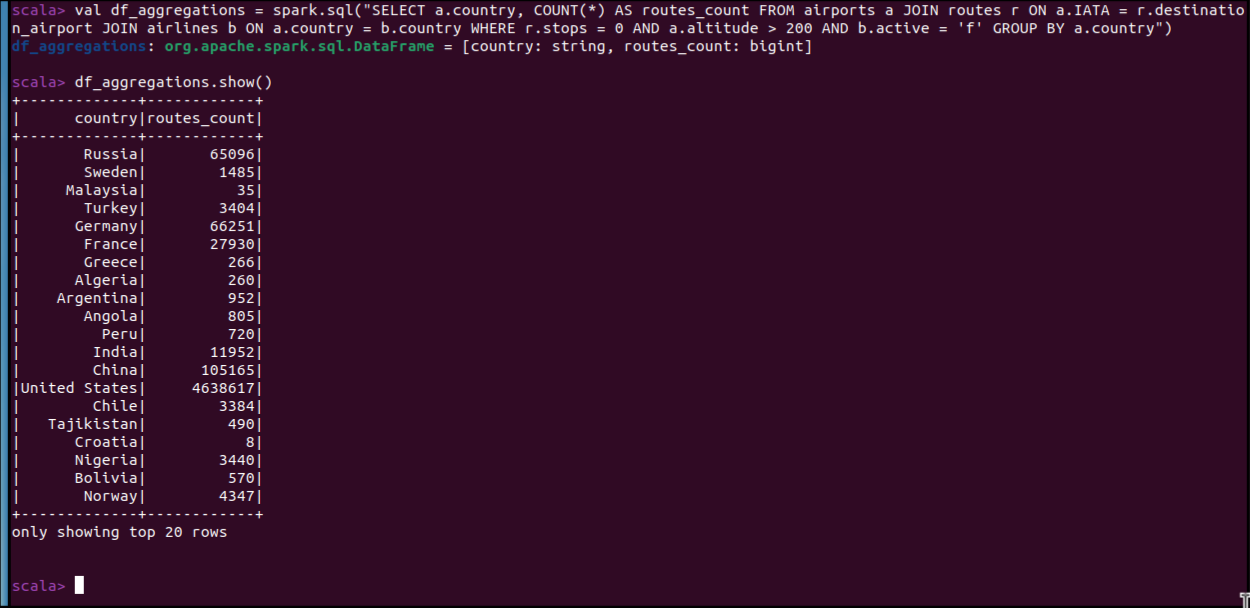
\includegraphics[width=0.8\textwidth]{figures/66.png}
    \caption{Resultado de la consulta de rutas sin paradas a destinos con altitud mayor a 200 metros por país con aerolíneas inactivas}
    \label{fig:consulta7}
\end{figure}

Ahora ya podemos guardar el dataframe en formato parquet en la ruta /practica/aggregations/ de HDFS:

\begin{lstlisting}[language=scala]
df_aggregations.write.format("parquet").save("hdfs://localhost:9000/practica/aggregations/") 
\end{lstlisting}

\begin{figure}[H]
    \centering
    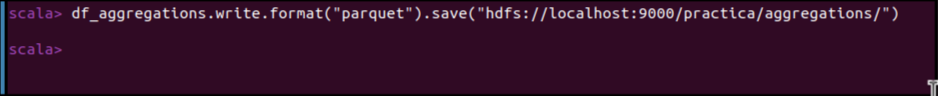
\includegraphics[width=0.8\textwidth]{figures/67.png}
    \caption{Guardado del dataframe en formato parquet en la ruta /practica/aggregations/ de HDFS}
    \label{fig:guardado}
\end{figure}

Ahora ya podemos consultar la tabla de agregaciones:

\begin{lstlisting}[language=scala]
spark.read.format("parquet").load("hdfs://localhost:9000/practica/aggregations/").show()
\end{lstlisting}

\begin{figure}[H]
    \centering
    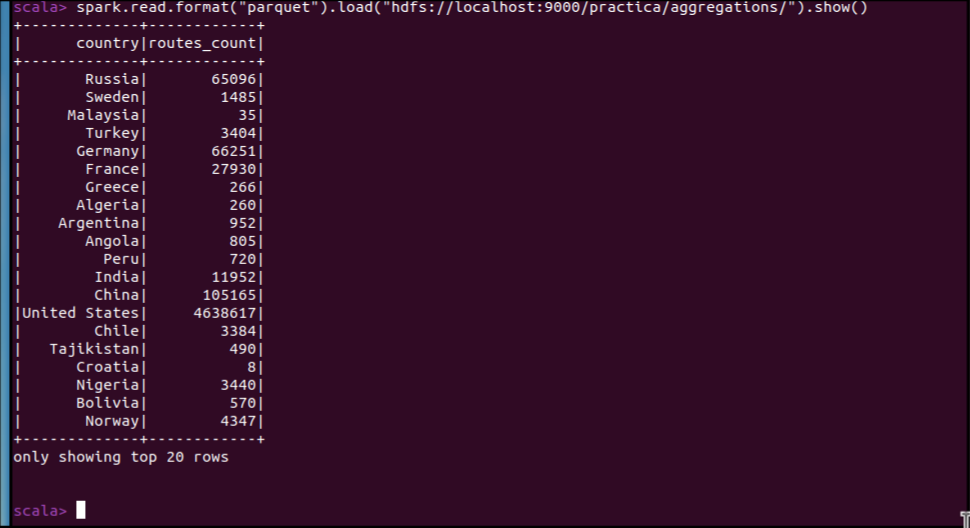
\includegraphics[width=0.8\textwidth]{figures/68.png}
    \caption{Resultado de la consulta de la tabla de agregaciones}
    \label{fig:carga-consulta}
\end{figure}
